\section{Operations Itself}

So then, we have seen that many supporting functions sit outside of operations management. What then sits inside this function?

Ultimately, as stated before, operations management is the portion of the business that is responsible for the transformational fuction of taking inputs and producing outputs that create value for customers. These customers can be retail customers, wholesale customers, or a combination of the two.

Operations learns about customer needs through the efforts of marketing and sales functions. Operations discovers its own financial limitations through supporting functions falling under the CFO. Operations gets this information through various channels, frequently under the auspices of an IT department. And operations works with supply chain management and logistics/shipping to ensure delivery to operations of necessary inputs and to the customer of the desired outputs.

Operations in manufacturing can be thought of as a sequence of micro-operational steps, each of which is its takes its own inputs and provides for transformation to an output. An auto manufacturer, for example, might take in steel sheets, and one process cuts them to size for a body panel molding process. These are output to that process, which accepts them as inputs. This molding process, has a customer demand based on the final target production, but also on what the subsequent micro-process is building.

Part of operations management is in driving efficiencies into this process. Often it can be the case that operations can off-load the actual production to a third-party supplier. Now, instead of receiving sheet metal and having to take it through each micro-step in transforming it to a fully  assembled car body, the manufacturer might simply work with the supply chain management team to contract for the JIT delivery of a specific sub-assembly. This can reduce costs and increase efficiency \parencite{tsayReviewProductionOperations2018}.

\section{The Future is Now}

With the increased technological advances in managing supply chains using AI systems, as well as massive technological advances in automated manufacturing systems, operations management in what is known as ``Industry 4.0'' is often more about managing a control of informational flow from a wide network of sensors and systems that manage a complex network of predominately outsourced suppliers, and sub-assembly producers working under the direction of an operations team running smart factories, which are often nothing more than final assembly points positioned to minimize shipping costs to customers \parencite{parenteProductionSchedulingContext2020}.

In this realm, operations and IT have merged with supply chain management to create what is effectively an AI driven assembly process where each sub-assembly is merely a supplied input to the final product. There is little, to no, actual manufacturing done by the operations department. Rather, operations in this instance transforms inputs into value through producing efficiency, design, scheduling, and coordination between the various involved departments and numerous sub-contractors.  Operations management will coordinate, with contract management and supply chain management, the properly timed delivery of sub-components for primary assembly. Then, products will be shipped for final assembly and customization immediately prior to delivery to the end customer.

The result is a fast, cost-efficient system of manufacturing and delivery where value is created not by the company's labor in transforming inputs through direct manufacturing, but by the company's ability to schedule and coordinate transportation and assembly across time and distance in order to minimize costs and maximize end-user value (see fig \ref{fig:i4})

\begin{minipage}{\linewidth}
  \makebox[\linewidth]{ % to center image}
    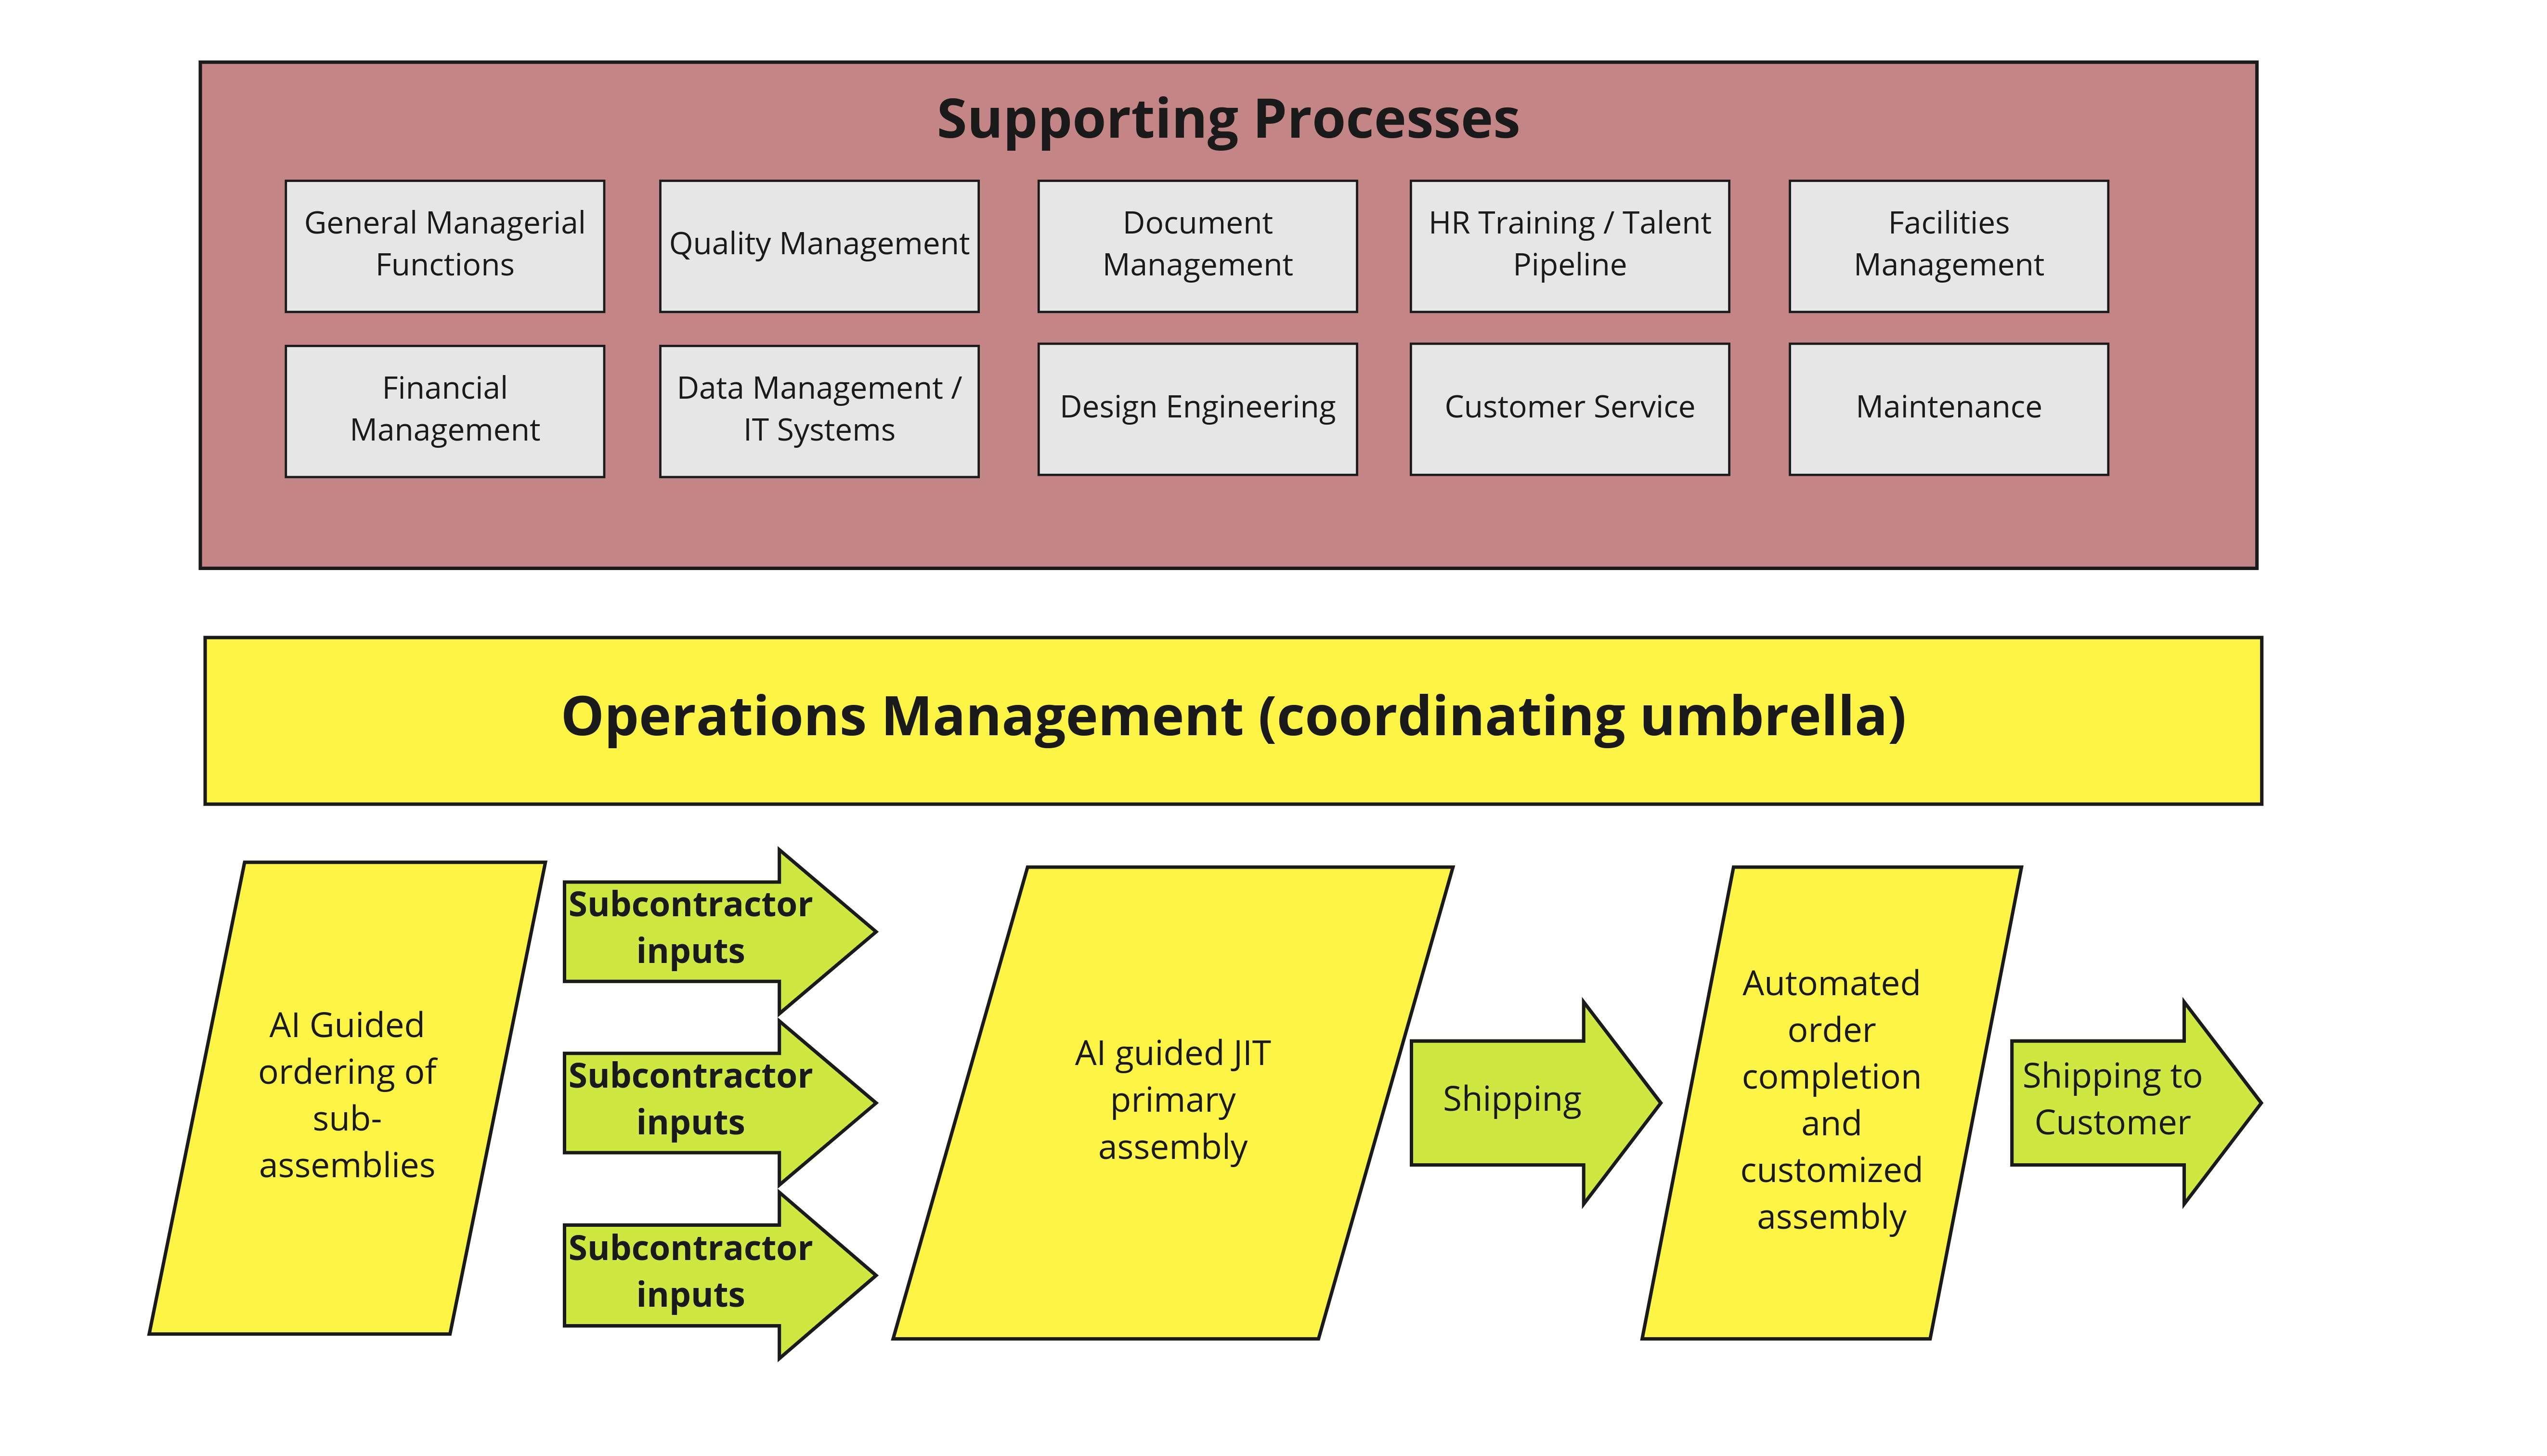
\includegraphics[width=6in]{img/om}}
    \captionof{figure}{Operations in Industry 4.0}
    \label{fig:i4}
\end{minipage}
